\documentclass{article}
\usepackage[utf8]{inputenc}
\usepackage{hyperref}
\usepackage{amssymb}
\usepackage{listings}
\usepackage{pgfplots}
\usepackage{geometry}
\usepackage{setspace}
\usepackage{graphicx}
\usepackage{float}
\usepackage{subfig}
\usepackage{microtype}

\doublespacing

\hypersetup{
    colorlinks=true,
    linkcolor=blue,
    filecolor=magenta,
    urlcolor=blue,
}
\usepackage{enumitem}% http://ctan.org/pkg/enumitem

\title{15-418 Final Project - Cachesim}
\author{Sam Flattery (sflatter) \and Brian Wei (bwei1)}
\date{\today}

\pgfplotsset{scaled y ticks=false}

\usepackage{xcolor}

% lstlistings stuff to make the code look nice
% https://www.overleaf.com/learn/latex/code_listing
\definecolor{codegreen}{rgb}{0,0.6,0}
\definecolor{codegray}{rgb}{0.5,0.5,0.5}
\definecolor{codepurple}{rgb}{0.58,0,0.82}
\definecolor{backcolour}{rgb}{0.95,0.95,0.92}

\lstdefinestyle{mystyle}{
    backgroundcolor=\color{backcolour},
    commentstyle=\color{codegreen},
    keywordstyle=\color{magenta},
    numberstyle=\tiny\color{codegray},
    stringstyle=\color{codepurple},
    basicstyle=\ttfamily\footnotesize,
    breakatwhitespace=false,
    breaklines=true,
    captionpos=b,
    keepspaces=true,
    numbers=left,
    numbersep=5pt,
    showspaces=false,
    showstringspaces=false,
    showtabs=false,
    tabsize=2
}

\lstset{style=mystyle}
\def\inline{\lstinline[language=C++, basicstyle=\ttfamily]}
% silence some weird warning
\pgfplotsset{compat=1.17}

\begin{document}

\maketitle

Project Website: \href{https://samflattery.github.io/cachesim}{https://samflattery.github.io/cachesim}

\section{Summary}
We implemented a cache simulator for a NUMA multiprocessor machine using directory based cache coherence and used the simulator to analyze the cache behavior of various synchronization lock implementations. We used Intel's \texttt{pin} program and a custom written pintool to gather memory access traces of different parallel programs written using these locks and compared their performance under the MSI, MESI and MOESI cache coherence protocols.  We created plots illustrating the differing cache performance of the locks and the differences between the protocols under various metrics such as cache hits/misses, main memory accesses and interconnect events.

\section{Background}
\subsection{NUMA}
NUMA (Non Uniform Memory Access) is a multiprocessing computer architecture in which memory access times depend on the proximity of the memory location to the processor requesting the access.  It is often used in distributed machines, as it means that processors have faster access to a subset of localized memory while still retaining the shared memory abstraction at the expense of occasional higher latencies when accessing memory further away.

\subsection{Cache Coherence and Directories}
In multiprocessor machines, where each processor has its own cache(s), lines of memory become replicated in multiple places, which means that different processors can observe different values for reads to the same memory address.  For example, if two processors have the same line of memory in each of their caches and one writes to it, the other will observe stale data on future reads.  In order to fix this problem, modern multiprocessor machines implement cache coherence systems within which caches communicate with each other under various coherence protocols to ensure each cache is aware of the current state of the line.

There are two main ways to implement cache coherence for a write-back, write-allocate cache - snooping-based and directory-based.  Snooping-based cache coherence is suited to smaller machines with relatively few processors, as it relies on the idea that coherence information is broadcasted on some system-wide interconnect to all other caches. However, this protocol doesn't scale very well to larger machines as the cost of the broadcasts scales with the number of processors.  Instead, large scale machines often use a directory-based implementation of cache coherence, in which a directory is used to track the set of caches that contain a line of memory. Under this scheme, coherence messages can be sent point-to-point to just the caches that need to be updated with new coherence information, which means the protocol scales well with the number of processors.  In NUMA machines, a distributed directory scheme is often used, meaning each NUMA node has its own directory which tracks the state of each line of memory in that node and these directories can communicate with each other to coordinate the system (see figure \ref{fig:numa}).

\begin{figure}[h]
\centering
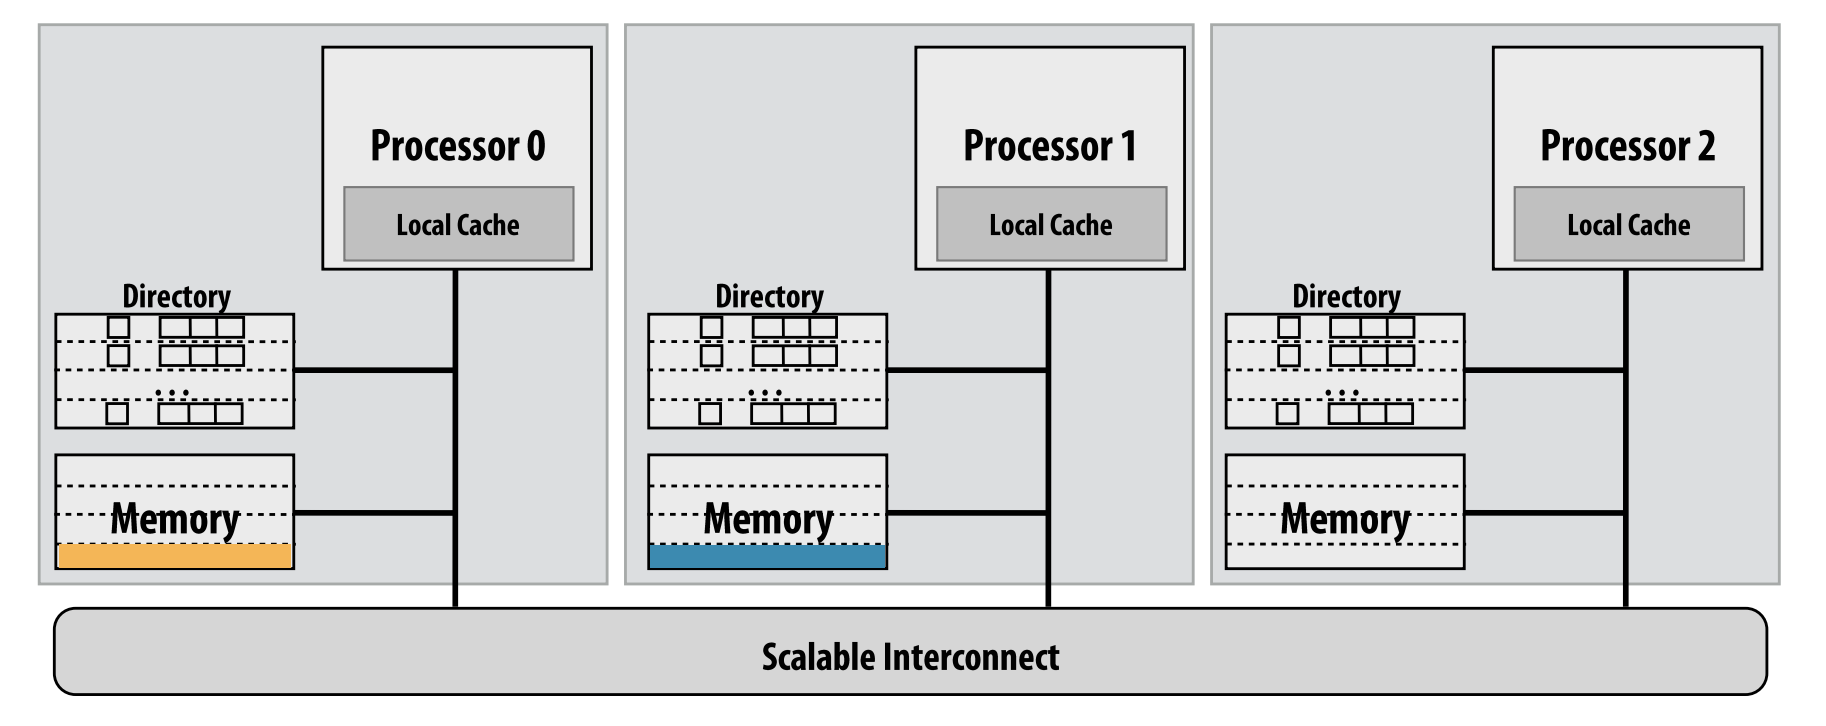
\includegraphics[width=\textwidth]{figures/numa.png}
\caption{A distributed directory on a NUMA system (\href{http://www.cs.cmu.edu/afs/cs/academic/class/15418-f20/public/lectures/11\_directorycoherence.pdf}{source})}
\label{fig:numa}
\end{figure}

For each line in memory, the directories maintain a set of $P$ presence bits, where $P$ is the number of processors in the system, as well as two bits representing the state of the line. A line can be in one of three states:
\begin{enumerate}
    \item \textbf{Uncached} (\texttt{U}) - the line is not present in any processor's cache
    \item \textbf{Shared} (\texttt{S}) - the line is in one or more caches and is clean
    \item \textbf{Exclusive/Modified} (\texttt{EM}) - the line is in exactly one cache who owns the data
\end{enumerate}

In order to implement the MOESI coherence protocol (discussed in \ref{subsec:protocols}), our directory also stores a cache identifier of which cache has the line in an owned state so the directory can forward read requests from other sharing caches to that cache.

The directory receives messages on the interconnect from caches, such as a \texttt{BusRd} when a cache wants to read a line or a \texttt{BusRdX} when a cache wants to read a line with the intention of writing to it (i.e. it needs exclusive access to the line) and responds to the messages by transitioning its state and sending its own coherence messages to the relevant caches.  The state transitions are illustrated in figure \ref{fig:dstates} below.

\begin{figure}[h]
\centering
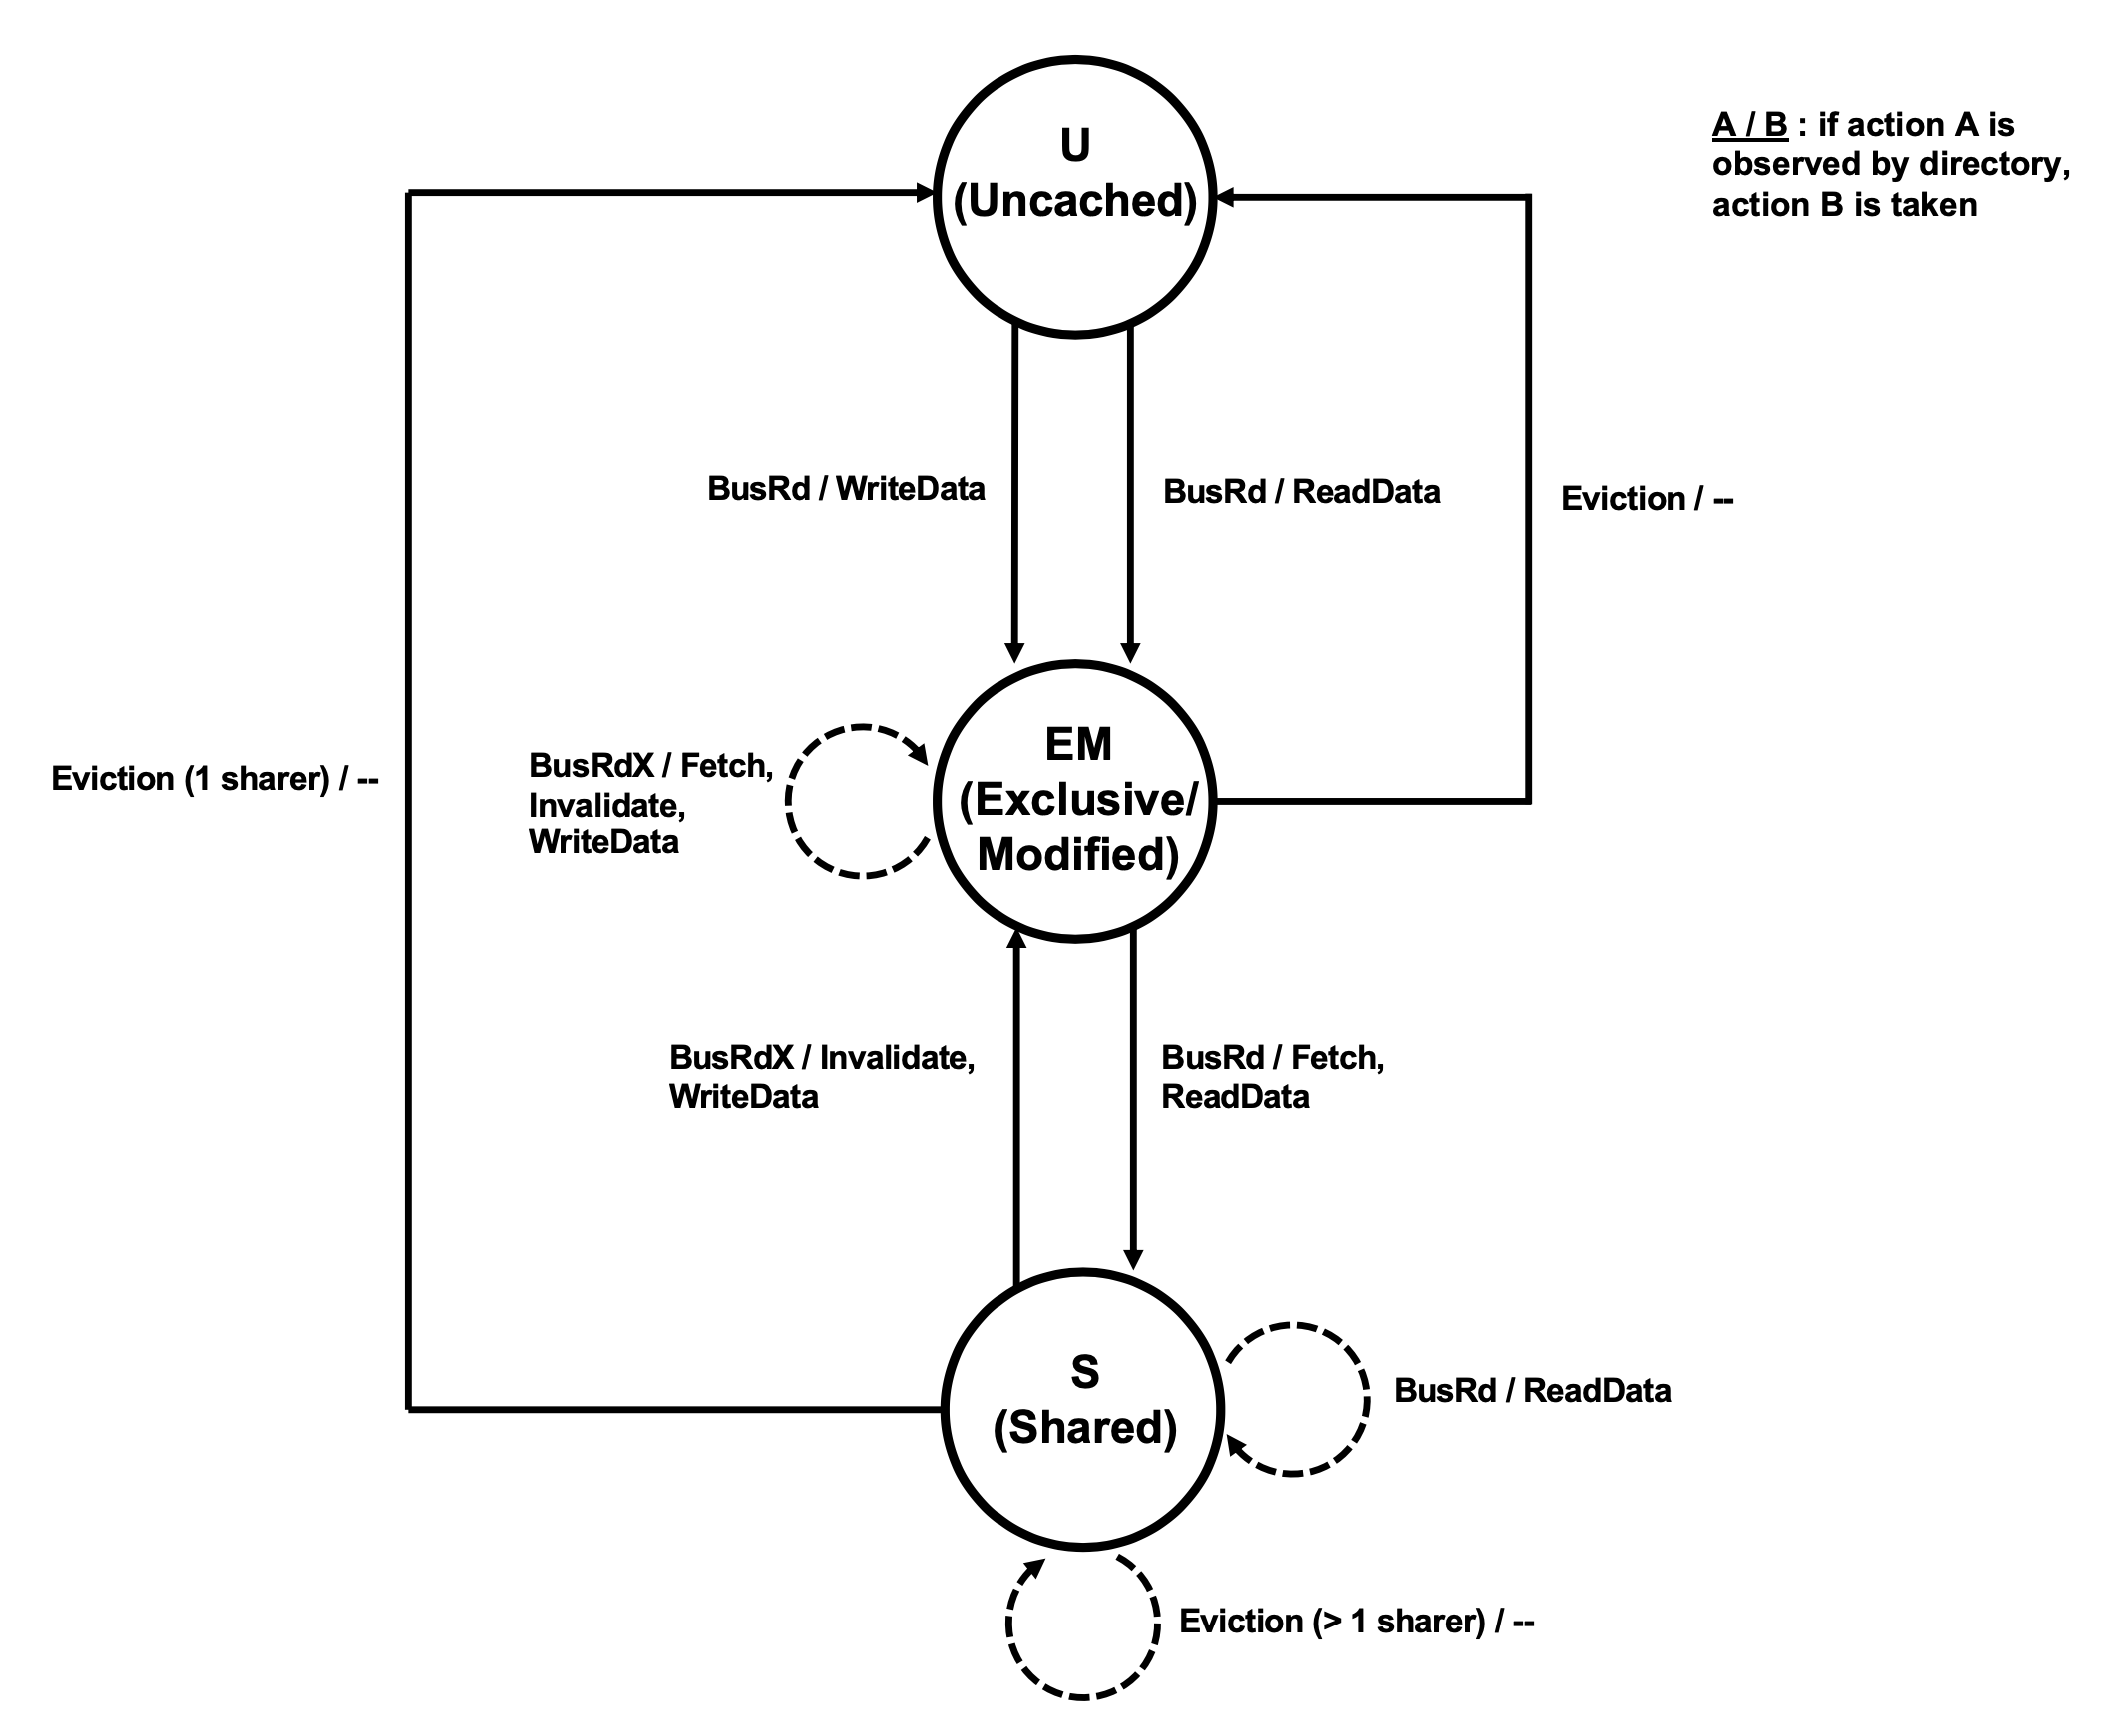
\includegraphics[width=.7\textwidth]{figures/dstates.png}
\caption{The state transitions of a directory}
\label{fig:dstates}
\end{figure}

\subsection{Cache Protocols}\label{subsec:protocols}
The caches also maintain a few bits of state for each line they have cached. Many different protocols are used here, but we chose to implement and analyse 3 - MSI, MESI and MOESI (each letter corresponds to a state the cache can be in).
\begin{itemize}
\itemsep 0em
    \item \textbf{M} (modified) - the cache holds a dirty modified copy of the line, no other caches have copies
    \item \textbf{O} (owned) - the cache holds exclusive rights to a line, other caches may read but only this cache may modify and must broadcast changes to all sharers
    \item \textbf{E} (exclusive) - the cache has the only copy of the line and the line is clean
    \item \textbf{S} (shared) - the cache is one of at least one other sharer of the line and the line is clean
    \item \textbf{I} (invalid) - the block is not valid in the cache and cannot be read/written
\end{itemize}
where the states in MSI are a subset of those in MESI, etc.  The cache lines transition between these states in response to events from the processor, as well as events received on the interconnect from the directories.  The state transition diagrams for the coherence protocols we implemented are presented below (the interconnect transactions are explained in tables \ref{table:cache_to_dir} and \ref{table:dir_to_cache}).

MSI requires two interconnect messages for the common case of reading an address and then writing to it (e.g. incrementing a variable). MESI helps to reduce this inefficiency by adding the \inline{E} state, which means that if a processors wants to do a read-write and no other processor is currently sharing the data, it will get an exclusive copy of the data for the read which can then be upgraded to a modified copy for free without any interconnect traffic.

\begin{figure}[H]
\centering
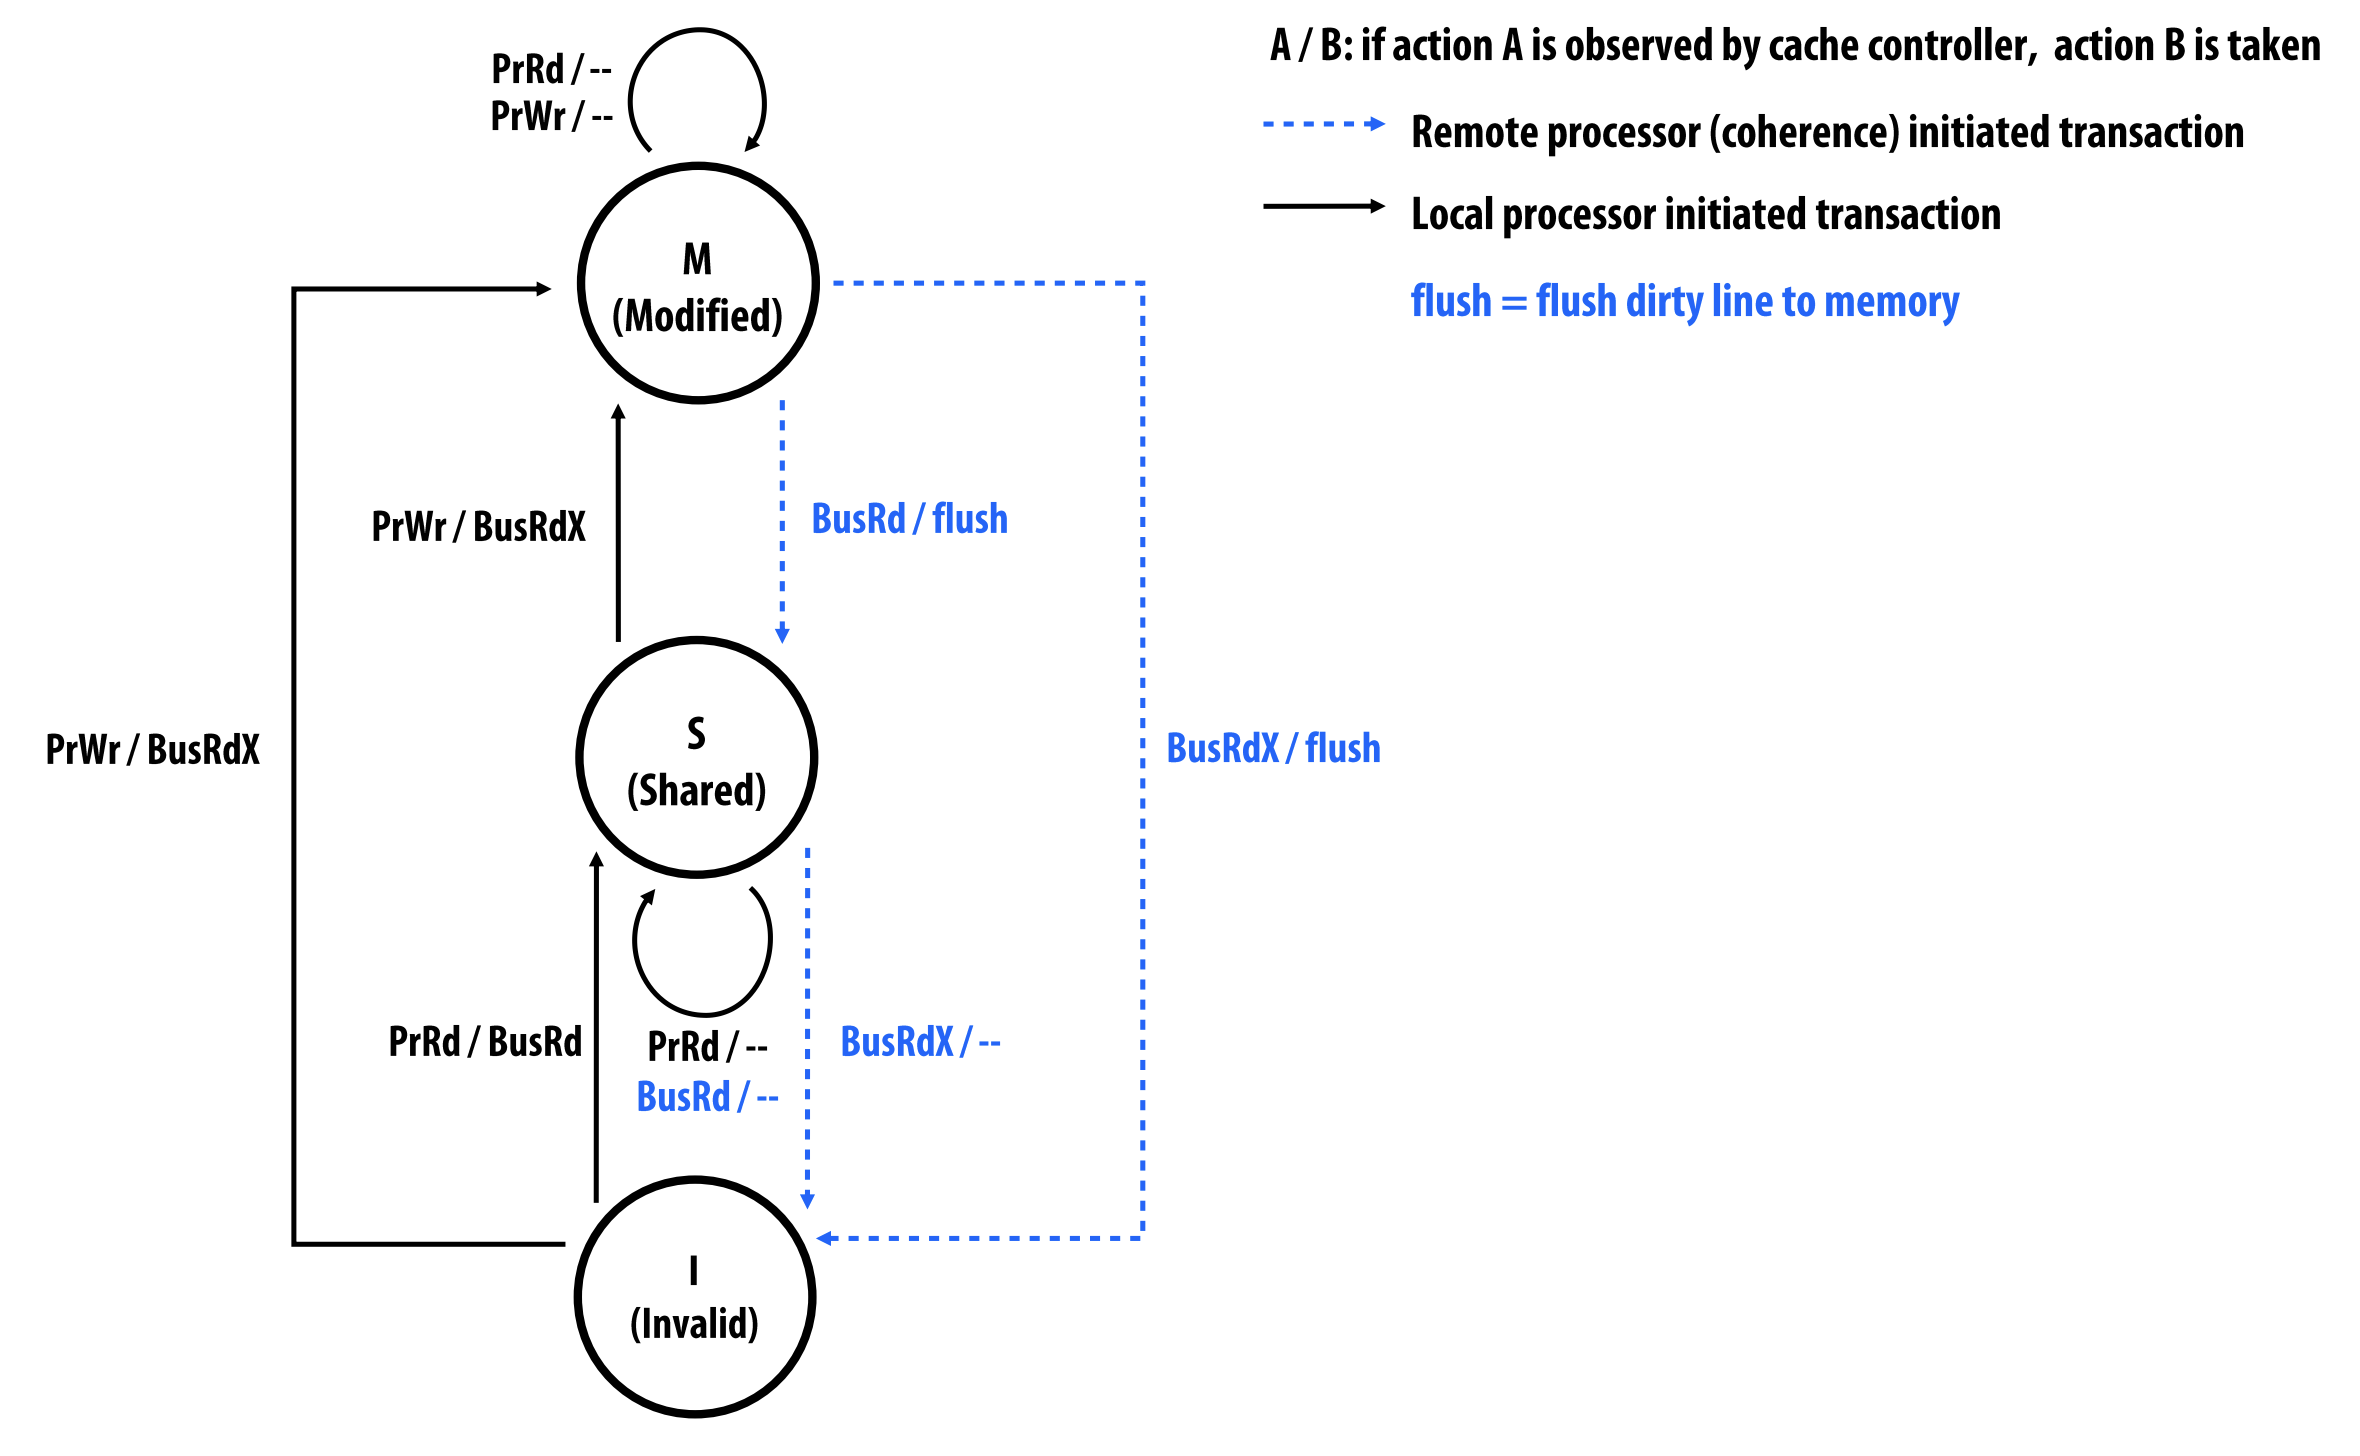
\includegraphics[width=.8\textwidth]{figures/msi.png}
\caption{The state transitions in MSI (\href{http://www.cs.cmu.edu/afs/cs/academic/class/15418-f20/public/lectures/10\_cachecoherence1.pdf}{source})}
\end{figure}


\begin{figure}[H]
\centering
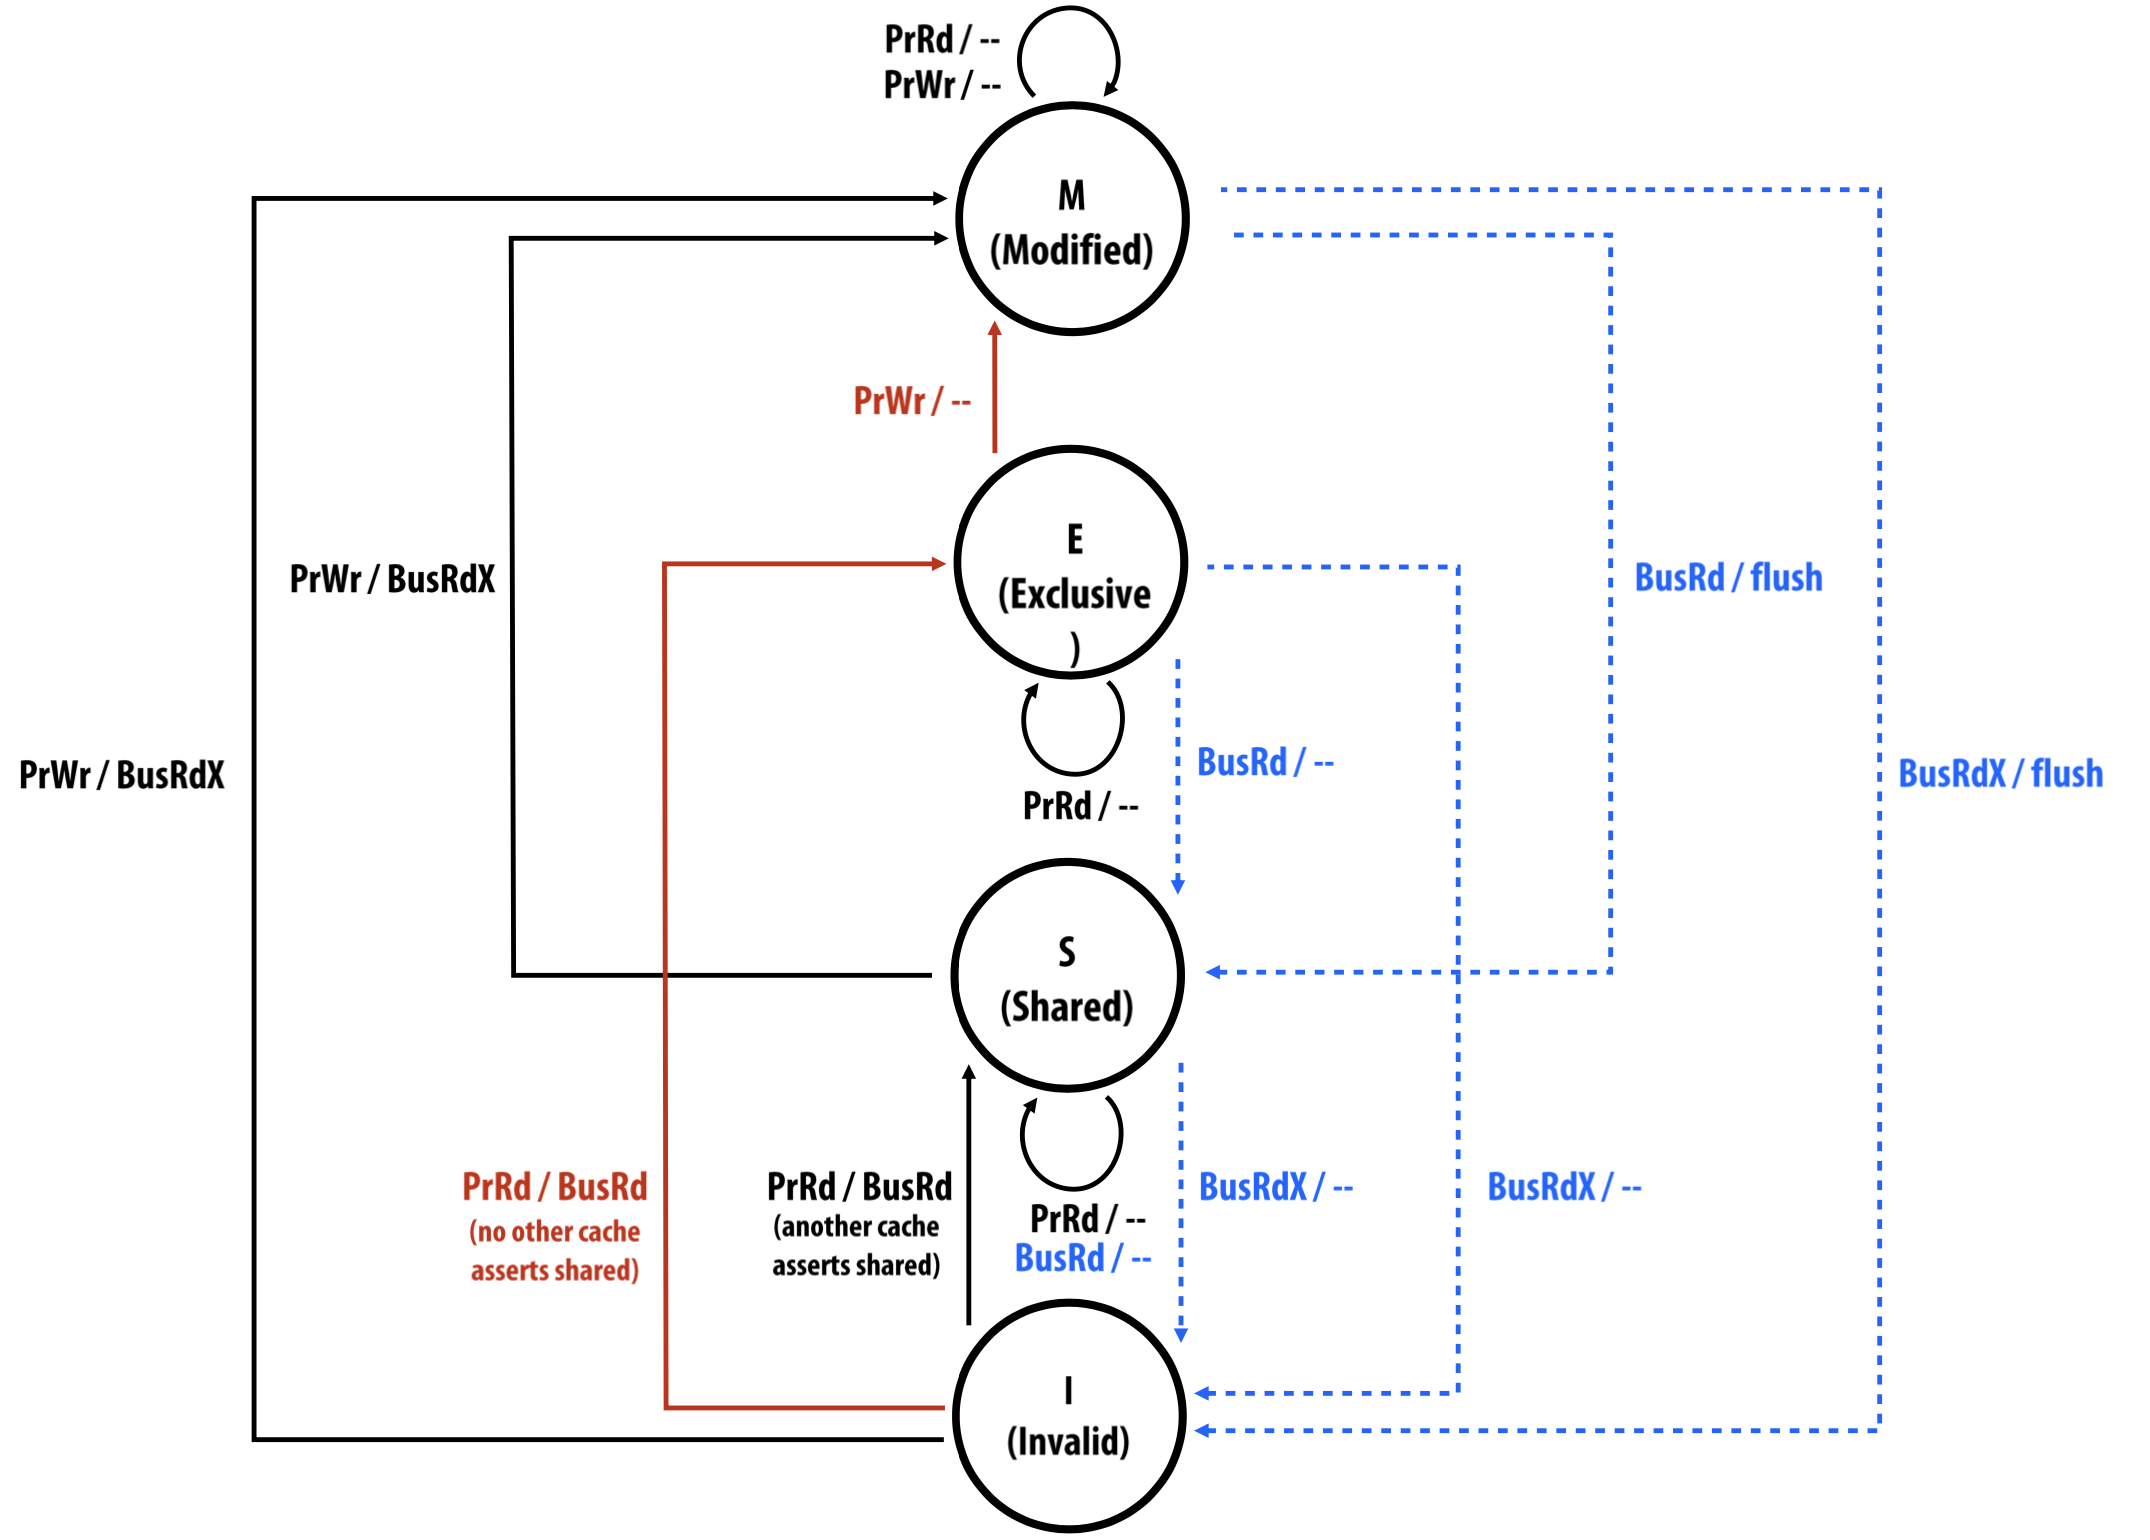
\includegraphics[width=.8\textwidth]{figures/mesi.png}
\caption{The state transitions in MESI (\href{http://www.cs.cmu.edu/afs/cs/academic/class/15418-f20/public/lectures/10\_cachecoherence1.pdf}{source})}
\end{figure}

The MOESI protocol operates very similarly to the MESI protocol, with the addition of the \inline{O} state.  This protocol reduces the number of memory writes necessary, as now when another CPU wants to read a dirty line, a flush is not necessary as the data is now sent over the interconnect directly from the owning cache.

\begin{figure}[H]
\centering
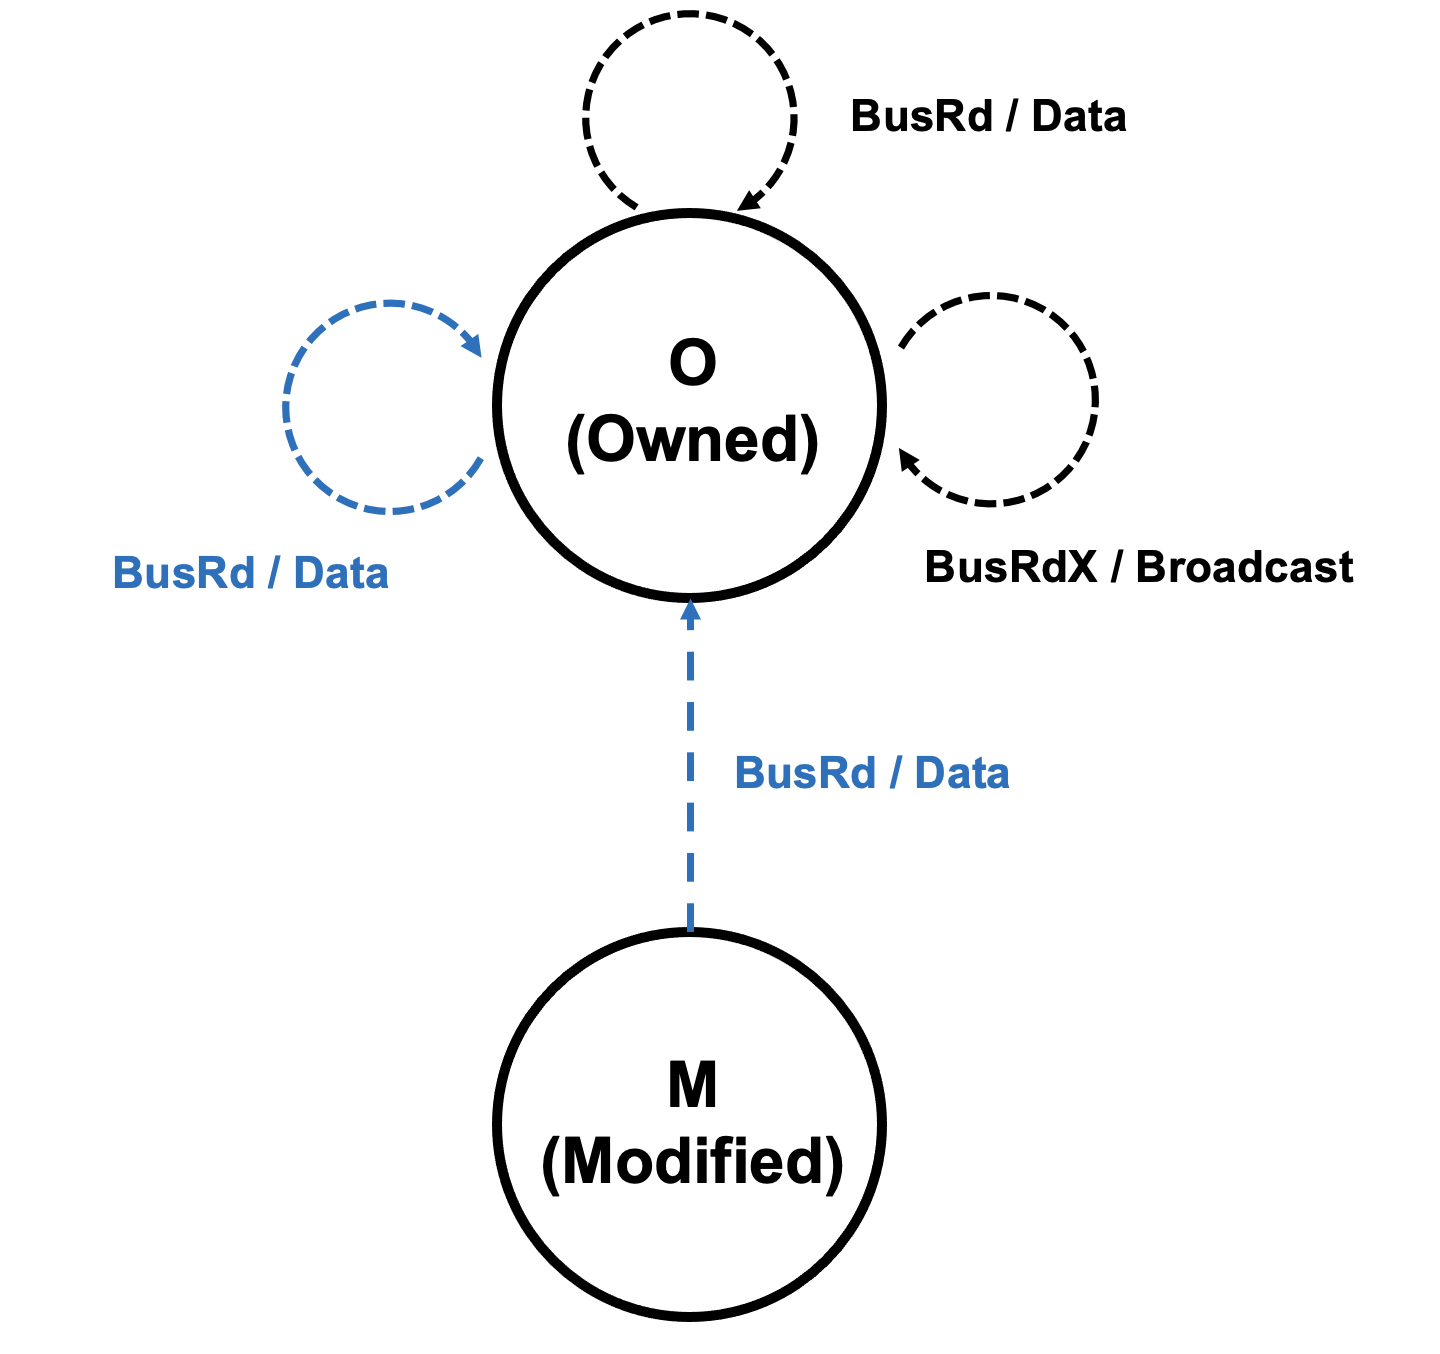
\includegraphics[width=.3\textwidth]{figures/moesi.png}
    \caption{The new state transitions in MOESI (other transitions remain the same as MESI)}
\end{figure}

\subsection{Locks}
In order to evaluate the cache simulator, we run the simulator on a large number of traces generated from running parallel programs. We chose to analyse several lock types, as locks serve as a fundamental aspect of synchronizing parallel programs and they exhibit interesting cache coherence behaviour as their memory can be highly contended.  We chose to implement the following types of locks to look for differences in their performance in various cache protocols:
\begin{itemize}
    \item {\bf test-and-set:} This lock relies on the atomic test and set instruction.  The lock will spin on the test and set instruction, checking repeatedly whether a variable is in a desired {\it unlocked} state and trying to set it to be {\it locked} if so.
    \item {\bf test-and-test-and-set:} This lock improves on the test-and-set lock by reducing the traffic on the interconnect by spinnning on a test while the lock is locked, then only attempting to acquire the lock with test-and-set when it knows the lock has been released.
    \item {\bf ticket lock:}  The ticket lock provides an improvement over the first two lock types for two reasons - fairness (by guaranteeing that locks are granted in the order they are requested) and fewer invalidations.  It results in fewer invalidations since only a read is required to acquire the lock, instead of a write in the test-and-test-and-set case, which means the only invalidations come from the release of the lock. It is implemented by maintaining a ticket number that each thread increments when it acquires the lock, and a serving number which is incremented when a thread releases the lock.  A thread then acquires the lock when its ticket number is equal to the serving number.
    \item {\bf array lock:} The array based lock is similar to the ticket lock in that it maintains fairness, while providing a further decrease in the amount of interconnect traffic.  To do so, the lock uses an array where a thread acquires the lock by waiting on an element ofthe array to be set to the unlocked state, and released the lock by setting the next element to the unlocked state. This lock can be further improved by having each array element padded to be on separate cache lines, which prevents false sharing.  The drawback of this lock is the space requirement, which is linear in the number of threads.
\end{itemize}

\section{Approach}

% describe pintool
\subsection{Pintool}
We used Intel's \texttt{pin} program to instrument the binaries of several parallel programs we had written in order to generate memory access traces of the programs.  \texttt{pin} allows you to insert callbacks into a compiled binary which run whenever certain instructions are executed.  In our case, we used \texttt{pin}'s built in \texttt{INS\_MemoryOperandIsRead} and \texttt{INS\_MemoryOperandIsWrite} functions to insert a callback after every memory read and write from the programs under analysis.

Our pintool creates a trace that looks like the following:
\begin{lstlisting}[numbers=none]
[CPU] [R/W] [Address] [NUMA Node]
1 R 0x7ffef17ecea8 0
2 W 0x7ffef17ecea0 1
3 W 0x7ffef17ece90 0
4 W 0x7ffef17ece88 0
\end{lstlisting}

We make the simplifying assumption here that each thread is running on a different physical CPU, which obviously is not always the case but it allows us to better analyse the programs we write since we get a more even distribution of work between the CPU cores.  We found when generating traces that even programs with high amounts of parallelism ran on only a few physical processors.

We also used a simple probabilistic method to decide which NUMA node an address resided on.  When running a program through pin, we will periodically read and parse the Linux proc filesystem's numa maps.  This provides information on various regions of memory and how many numa nodes they are mapped to.  This information is not precise however; it will only indicate the number of pages in the region that belong to each node (e.g. if the region has 20 pages, it may indicate there are 8 on node 0 and 12 on node 1).  Whenever we encounter an address on a previously unseen page, we probabilistically assign that page to one node from the given region based on the ratios.  This information is saved so that future accesses to the same page are given its numa node consistently.

\subsection{Usage}
Our simulator is run with the following parameters:
\begin{lstlisting}[numbers=none]
-t <tracefile>: name of memory trace to replay
-p <processors>: number of processors used to generate trace
-n <numa nodes>: number of NUMA nodes used to generate trace
-m <MSI | MESI | MOESI>: the cache protocol to use
-s <s>: number of set index bits (number of sets = 2^s)
-E <E>: associativity (number of lines per set)
-b <b>: number of block bits (number of blocks = 2^b)
-v: verbose output that displays trace info
-a: display aggregate stats
-A: display aggregate stats not including processor 0
-i: display individual stats (i.e.) per cache, per NUMA node
-h: help
\end{lstlisting}

The user specifies how many processors and NUMA nodes the trace was generated with, as well as the protocol to use and the properties of the cache (i.e.e how many blocks per set, the size of the blocks and how many sets per cache). These default to \texttt{s = 6}, \texttt{b = 6}, \texttt{E = 8}, giving an 8-way associative 32kB cache which is the configuration of an Intel L1 cache.

The user can also specify the output of the simulator using the \texttt{-Aaiv} flags. The \texttt{-v} flag gives a verbose output which prints the interconnect events that are happening on a per memory access basis. The \texttt{-a -i} flags print stats after running the program on an aggregate or per cache level.  We noticed that for the smaller programs that it was feasible to generate pin traces for, thread 0 had far more activity than the other threads since it was being used to set up the program and create other threads, etc., so we included the \texttt{-A} flag to give aggregate stats without the first thread's stats being included. These flags can be used together to get the entire output of the program.

\subsection{Stats and Latencies}
The entire list of stats the simulator collects are shown below:
\begin{lstlisting}[language=C++, numbers=none]
struct Stats {
  size_t hits_;                 // cache hits
  size_t misses_;               // cache misses
  size_t flushes_;              // flushes from cache to memory
  size_t evictions_;            // evictions from cache
  size_t dirty_evictions_;      // evictions of dirty lines from cache
  size_t invalidations_;        // invalidations due to coherence
  size_t local_interconnect_;   // intra-NUMA node interconnect messages
  size_t global_interconnect_;  // inter-NUMA node interconnect messages
  size_t memory_reads_;         // reads of main memory
  size_t memory_writes_;        // writes to main memory
}
\end{lstlisting}

Our simulator also has a simple timing model, in which it uses fixed latencies for different events. The default latencies are shown in table \ref{table:latencies}, but these are adjustable by editing the \inline{latencies.h} file which defines these as constants. The latencies we used are based off latencies we found online for commonly used interconnects and memory systems.  The NUMA distance on \inline{andrew} is 2, so we set the global interconnect latency to be twice the local.
\begin{table}[H]
    \centering
    \begin{tabular}{| c | c |}
        \hline
        \textbf{Event} & \textbf{Latency} \\
        \hline \hline
        \textbf{Cache Access Latency} & $1ns$ \\
        \hline
        \textbf{Memory Access Latency} & $100ns$ \\
        \hline
        \textbf{Local Interconnect Latency} & $1ns$ \\
        \hline
        \textbf{Global Interconnect Latency} & $2ns$ \\
        \hline
    \end{tabular}
    \caption{Default Latencies}
    \label{table:latencies}
\end{table}

The combination of these latencies and the stats we collect allows us to get rough estimates of how long the memory accesses of programs should take.  We present the latency reports as part of the output when the user runs the program with stat reporting enabled.

\subsection{The Architecture}
We used C++ to write the simulator for a few reasons.  Firstly, the traces are very large ($\sim$100MB+) so we needed a performant language to get through the traces in a reasonable amount of time.  Secondly, we are modeling a lot of physical objects such as caches and directories, so it allowed us to encapsulate these objects into classes which made them a lot easier to work with than if we had used C.  It also meant we could reduce repetition in our code by doing things like having an abstract cache block class which we could inherit from to model other block types. The simulator is divided into 5 main classes - \inline{NUMANode}, \inline{Cache}, \inline{Directory}, \inline{Interconnect}, and \inline{CacheBlock}.

Given arguments about how many processors are in the node and what coherence protocol is being used, a \inline{NUMANode} is responsible for setting up a \inline{Directory}, \inline{Interconnect}, and one or more \inline{Cache}s. The main function reads the trace file and sends the reads/writes to the relevant \inline{NUMANode} which passes them on to the correct cache.  It is also responsible for aggregating stats from all entities in the node once the trace has been ran.

The \inline{Interconnect} class holds the logic for communicating between \inline{Cache}s and their \inline{Directory}, as well as between different \inline{NUMANode}s.  It keeps track of how many messages have been sent from a \inline{Cache} to a \inline{Directory} and vice versa, as well as how many messages have been sent between NUMA nodes which allows us to account for the different latencies of the inter- vs intra-node messages. The full list of interconnect messages the simulator supports are shown below in tables \ref{table:cache_to_dir} and \ref{table:dir_to_cache}.
\begin{table}[h]
    \centering
    \begin{tabular}{| l | l | p{.5\linewidth} |}
        \hline
        \textbf{Message Type} & \textbf{Data Sent} & \multicolumn{1}{| c |}{\textbf{Reason}} \\
        \hline \hline
        \textbf{BusRd} & Address & Cache wants to read line at the given address \\
        \hline
        \textbf{BusRdX} & Address & Cache wants to write line at the given address \\
        \hline
        \textbf{Data} & Cache line & Cache is responding to directory request to fetch data at some address (usually because the cache has a exclusive modified copy and another cache wants to read it) \\
        \hline
        \textbf{Eviction} & Address & Cache has evicted the data at the given address and thus is no longer sharing it \\
        \hline
        \textbf{Broadcast} & Address, cache line & In MOESI, when a cache writes to a line it owns it must broadcast the data to all caches that are sharing that line, so notify the directory to do so \\
        \hline
    \end{tabular}
    \caption{Cache $\rightarrow$ Directory Messages}
    \label{table:cache_to_dir}

    \bigskip

    \begin{tabular}{| l | l | p{.5\linewidth} |}
        \hline
        \textbf{Message Type} & \textbf{Data Sent} & \multicolumn{1}{| c |}{\textbf{Reason}} \\
        \hline \hline
        \textbf{ReadData} & Exclusive bit, cache line & Send a cache back a cache line after it asked to read it, and tell the cache if it has an exclusive copy of it \\
        \hline
        \textbf{WriteData} & Cache line & Send a cache back a cache line after it asked to write it \\
        \hline
        \textbf{Fetch} & Address & Request that the cache sends its data and transitions to a sharing state (or in MOESI, just send data and remain in owning state) \\
        \hline
        \textbf{Invalidate} & Address & Invalidate a line in a sharing cache after a different cache got exclusive access to the line \\
        \hline
    \end{tabular}
    \caption{Directory $\rightarrow$ Cache Messages}
    \label{table:dir_to_cache}
\end{table}

We model a \inline{Cache} as follows:
\begin{lstlisting}[language=C++]
struct Set {
  Set(int associativity, Protocol protocol);
  std::vector<CacheBlock*> blocks_;
};

class Cache {
 public:
  Cache(int id, int numa_node, int s, int E, int b, Protocol protocol=MESI);
 private:
  std::vector<Set> sets_;
}
\end{lstlisting}

Where the relevant \inline{CacheBlock} type is constructed to make up the \inline{Set} based on what protocol is specified (i.e. MSI/MESI/MOESI), and $|$\inline{sets_}$|$  = $2^\texttt{s}$, $|$\inline{blocks_}$|$  = \inline{E}.  The \inline{Cache} class is responsible for servicing read/write requests to a given address, updating the state of the \inline{CacheBlock}s and communicating with the \inline{Directory} when necessary to send coherence messages.

The \inline{Directory} maintains the current state of every line of memory in the \inline{NUMANode}.  It responds to coherence messages from \inline{Cache}s by updating its internal state and sending more coherence messages to other caches across the system. For example, upon receiving a \inline{BusRdX}, it would send an \inline{Invalidate} message to all other caches sharing that line, so they have to re-request a fresh copy of the line on their next read.
\begin{lstlisting}[language=C++]
struct DirectoryLine {
  DirectoryState state_;        // U, S, EM
  std::vector<bool> presence_;
  int owner_;                   // in MOESI, the cache with the block in O state
};

// defines a mapping { memory line address -> DirectoryLine }
class Directory {
 private:
  std::unordered_map<unsigned long, DirectoryLine *> directory_;
};
\end{lstlisting}

\inline{CacheBlock} is an abstract class from which the three block types we implemented - \inline{MSIBlock}, \inline{MESIBlock}, and \inline{MOESIBlock}, inherit from.  These classes are responsible for storing the state of the block based on what protocol they implement, and correctly transitioning between states after being read/written. After reads/writes, they return the interconnect message that should be sent to the \inline{Directory} based on what their new state is. They keep stats on the events that have happened, such as hits, misses, evictions, invalidations etc.

\subsection{Programs}
\subsubsection{Locks}
In order to implement the lock programs, we took advantage of the atomic types from the C++ standard library.  This provided an easy way to use atomic operations such as increment and exchange without the need to explicitly write assembly code.

The test-and-set and test-and-test-and-set locks are implemented using {\tt atomic\_exchange} function.  This is essentially a test-and-set operation that we can perform on the lock variable.  In the implementation of the ticket lock, two counters are used -- one to indicate the next ticket and another to indicate the ticket currently being {\it served}.  Atomic operations of load, store, and increment are used to implement this as a thread needs to increment to set the next ticket, load the current ticket as it waits, and store the new current ticket when it unlocks.

The array based lock is implemented with an array size of 128.  This number was chosen arbitrarily, but is sufficient for supporting a reasonable large number of threads.  In a typical array based lock implementation, an atomic circular increment is used (i.e. perform {\tt x := (x + 1) \% n} atomically).  This is both difficult to implement and expensive to run.  Instead, we use an atomic fetch and increment followed by a non-atomic modulo.  All later indexing into the array likewise uses a modulo.  Since the index into the array becomes ever increasing, this can lead to correctness issues after billions of uses of the lock.  However, this version was sufficient for our tests and easier to implement.  We have an additional implementation of the lock where each array element is aligned and on separate cache lines.

\subsubsection{Evaluation}
We wrote a simple program to evaluate the locks.  In the program, threads repeatedly acquire the lock, increment a shared variable, and release the lock.  In order to artificially create more contention, we have each thread sleep for one second while holding the lock.  In order to balance the amount of time it took to run the traces and obtaining more data, we chose for each thread to make 10 increments.  We ran this program with each lock type with 2, 4, 8, 16, and 32 threads.

To evaluate with more realistic programs, we also implemented a simple concurrent binary search tree which allows for insertions only.  The general approach for this was to lock two nodes of the tree at a time as it traversed down to find where to insert.  To balance run time, amount of data, and managing very large file sizes, we had each thread make 100 insertions of random integers.  This was done with each lock type and 8 threads.

The main thread in both of these programs was just responsible for spawning and joining threads and did not perform the locking/unlocking computation done by the children threads.  This was intentional, as the work done by thread 0 to set up the program was substantially more expensive than the simple operations every other thread was performing with the locks, which lead to the stats collected about the locks being diluted greatly by the large number of operations in setup.  We added the {\tt -A} flag in order to isolate the stats about the lock performance.

\section{Results}

We wrote a script to generate plots for all of the metrics we collected, comparing lock types as well as cache coherence protocols. The most interesting findings are presented below.

\subsection{Test-and-Set Locks}
One of the most striking findings was how poorly regular test-and-set locks performed relative to the other locks.  The cause for this difference in performance is due to the cache coherence behaviour of the lock. Since it tries to perform a test-and-set every time it tries to see if the lock is available (requiring an exclusive copy of the line), there is an invalidation on every lock acquisition attempt.  This is seen in figure \ref{fig:tsbad} which shows that the invalidations and interconnect traffic between NUMA nodes is orders of magnitude higher than all other locks. This resulted in up to $\sim$10x slowdown on larger processor counts (see figure \ref{fig:speeds}) for test and set locks compared to the next slowest lock, as the invalidations meant that main memory had to be accessed frequently which is expensive compared to cache accesses.

\begin{figure}[h]%
    \centering
    \subfloat[\centering Invalidations]{{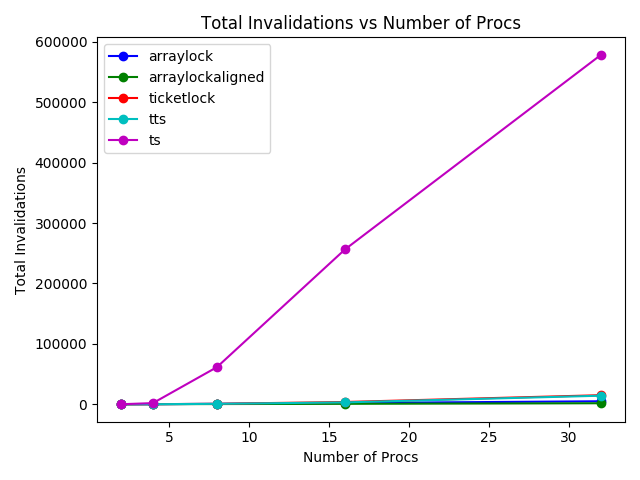
\includegraphics[width=.45\textwidth]{figures/ts_inval.png}}}%
    \qquad
    \subfloat[\centering Interconnect]{{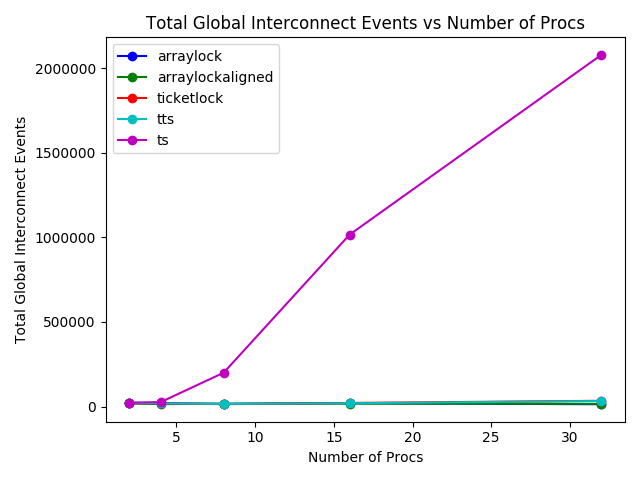
\includegraphics[width=.45\textwidth]{figures/ts_inter.png}}}%
    \caption{Test-and-Set Performance (MESI)}
    \label{fig:tsbad}
\end{figure}

\subsection{Highest Performance}
Firstly, it's worth noting the difference in the number of reads/writes necessary to implement each lock, because this varies between the locks, with the simpler test-and-set based locks performing $\sim20\%$ fewer instrutions than the arraylock and ticketlock (see figure \ref{fig:ops}). Our simulation showed that this made a big difference, with more cache-performant locks having slower estimated times due to this overhead.

\begin{figure}[h]
\centering
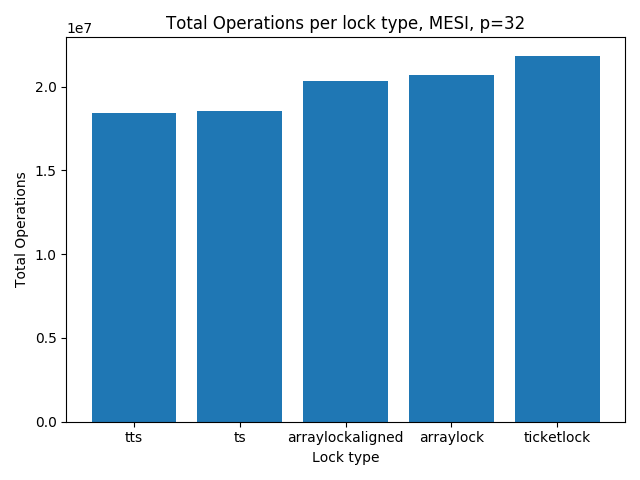
\includegraphics[width=.5\textwidth]{figures/ops.png}
\caption{Total operations of each lock type}
\label{fig:ops}
\end{figure}

From our comparisons, the fastest lock was the aligned arraylock.  Figure \ref{fig:speeds} below shows the estimated runtimes the simulator calculated for each of the programs, which is based off the stats collected and our estimated latencies.

\begin{figure}[h]%
    \centering
    \subfloat[\centering With \inline{ts_lock}]{{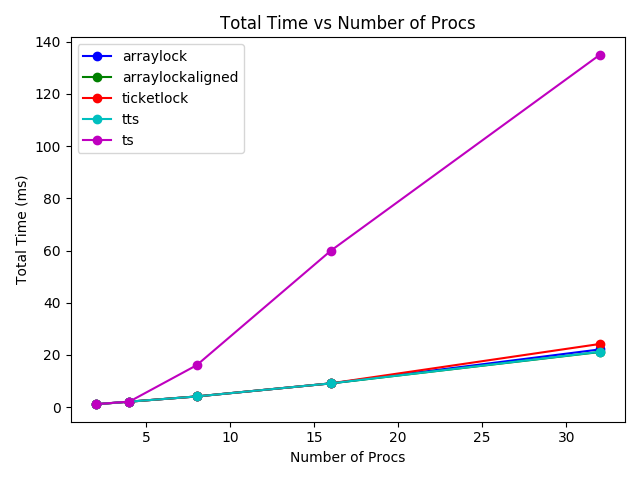
\includegraphics[width=.45\textwidth]{figures/ts_time.png}}}%
    \qquad
    \subfloat[\centering Without \inline{ts_lock}]{{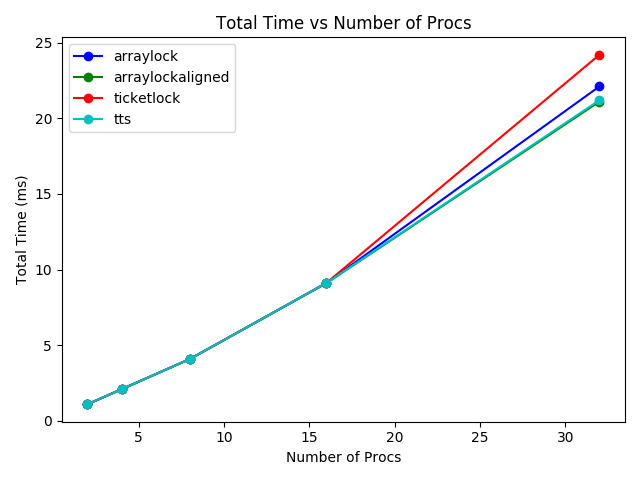
\includegraphics[width=.45\textwidth]{figures/no_ts_time.png}}}%
    \caption{Total Estimated Program Time (MESI)}
    \label{fig:speeds}
\end{figure}

The aligned arraylock far outperformed any other locks in terms of having fewer memory reads due to missing infrequently in the cache. It also had the fewest number of invalidations due to the fact that it has $O(1)$ invalidations per cache per lock release while ticketlock has $O(P)$ and test-and-test-and-set has $O(P^2)$. It's also interesting to see the implications of false sharing as demonstrated by the difference between the aligned and unaligned arraylocks, with the unaligned lock having $\sim$2x as many invalidations and memory reads as its aligned counterpart. The difference in performance in these areas is illustrated below in figure \ref{fig:arraylock}.

The test-and-test-and-set lock (tts lock) performed second best even though its cache performance was far worse than the unaligned arraylock, which is due to the fact that it requires fewer memory operations and thus less time to acquire the lock (see figure \ref{fig:ops}.  The ticketlock suffers from both relatively many operations as well as poor cache performance, so it performs the worst.  An interesting thing to note is that while theoretically the tts lock has $O(P^2)$ invalidations and interconnect traffic, we saw $O(P)$ in our test programs. This was due to the fact that upon the release of the lock, all copies of the lock are invalidated.  Since threads require an exclusive ownership of the line to do the test-and-set, at most one cache's line is invalidated per test-and-set attempt since all threads try to test-and-set at the same time.

\begin{figure}[h]%
    \centering
    \subfloat[\centering Invalidations]{{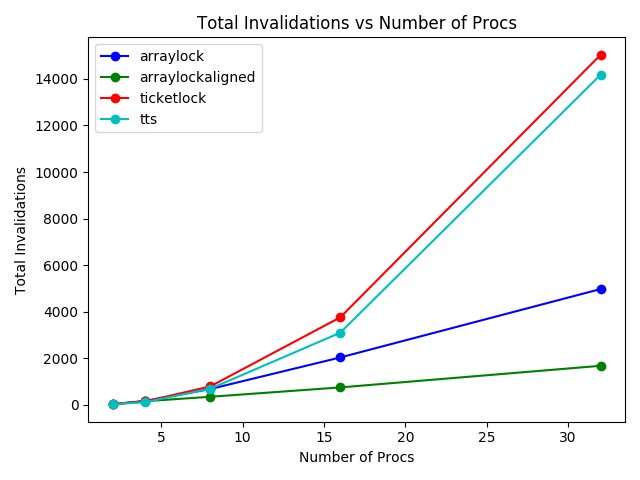
\includegraphics[width=.45\textwidth]{figures/no_ts_invalid.png}}}%
    \qquad
    \subfloat[\centering Memory Accesses]{{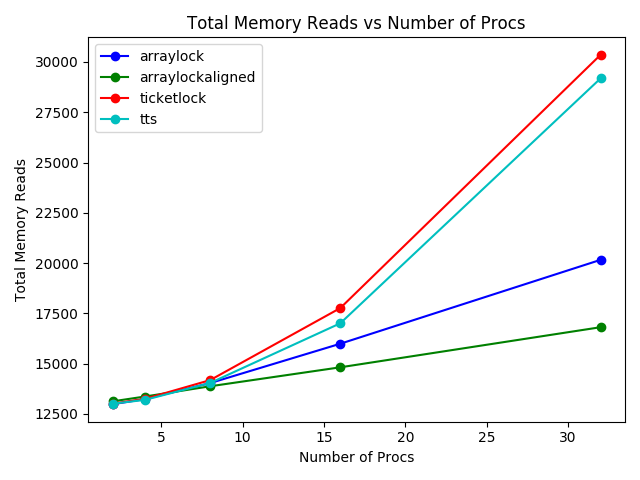
\includegraphics[width=.45\textwidth]{figures/no_ts_mem.png}}}%
    \caption{Performance Characteristics of Arraylock (MESI)}
    \label{fig:arraylock}
\end{figure}

\subsection{Cache Coherence Protocols}

We also compared performance of the cache coherence protocols we implemented (MSI, MESI, MOESI) and found some interesting results. The difference between MSI and MESI was most clearly exhibited by the aligned arraylock, where the benefits of the exclusive state were seen.  As figure \ref{fig:mesi} shows, the lock had a constant number of fewer reads regardless of the number of processors.  The reason for this is when a thread wants to lock the lock, it must increment the index, which is a read-write operation.  In MSI, this results in a \inline{BusRd}, during which memory is read, and then a \inline{BusRdX}, during which memory is read again before sending the \inline{WriteData} message.  However, in MSI, the processor can get an exclusive copy of the line after the first \inline{BusRd} and not have to send a \inline{BusRdX} the second time.

\begin{figure}[h]
\centering
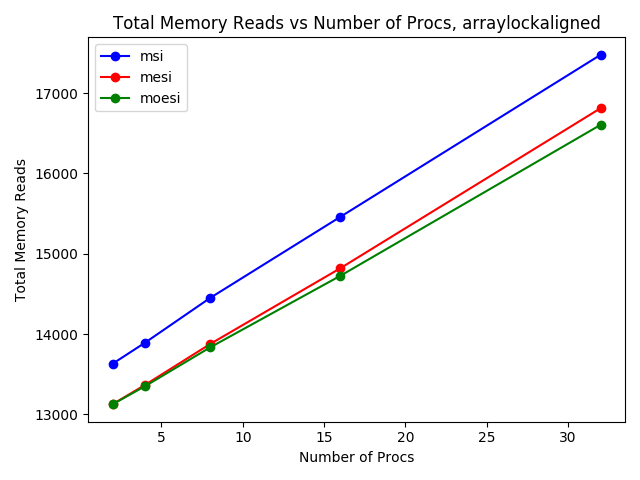
\includegraphics[width=.5\textwidth]{figures/arraylock_mem.png}
\caption{MESI performs better than MSI on \inline{arraylock_aligned}}
\label{fig:mesi}
\end{figure}

For the less cache-friendly locks such as ticketlock, we observed noticeable differences between MOESI and the two other protocols.  As shown in figure \ref{fig:moesi}a), there was greater interconnect traffic with MOESI than the other protocols, which is explained by figure \ref{fig:moesi}b), which shows at higher processor counts, MOESI is giving a 50\% reduction in memory accesses.  The reason for this is that the owning cache is serving memory lines to the other caches instead of flushing to memory, which causes the interconnect traffic to increase. Since interconnect events are far cheaper than memory accesses (100x cheaper in our model), this shows the benefits of the MOESI protocol.

\begin{figure}[H]%
    \centering
    \subfloat[\centering Interconnect Traffic]{{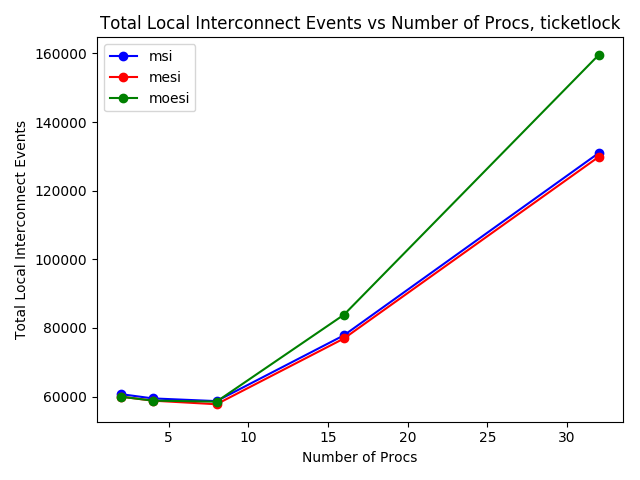
\includegraphics[width=.45\textwidth]{figures/ticketlock_inter.png}}}%
    \qquad
    \subfloat[\centering Memory Reads]{{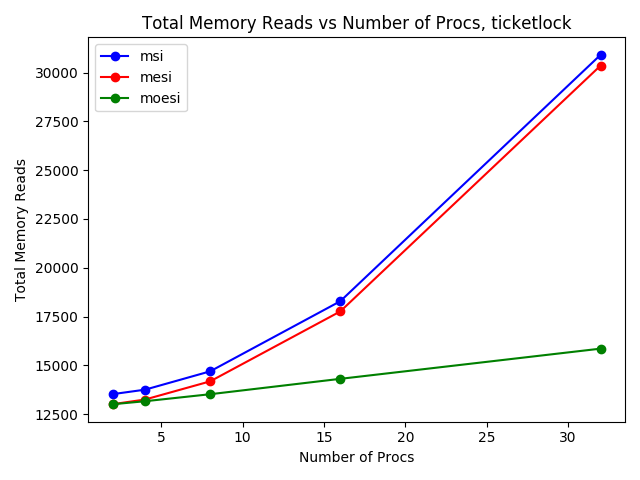
\includegraphics[width=.45\textwidth]{figures/ticketlock_mem.png}}}%
    \caption{Performance of MOESI vs MESI/MSI}
    \label{fig:moesi}
\end{figure}

We were also able to observe this behaviour in other programs.  In the binary search tree program with the test-and-set lock, we were able to see that the MOESI protocol led to substantially fewer memory accesses compared to other protocols (figure \ref{fig:bst}), as the owning cache can again serve the data instead of going to memory which leads to a speedup.

\begin{figure}[h]
\centering
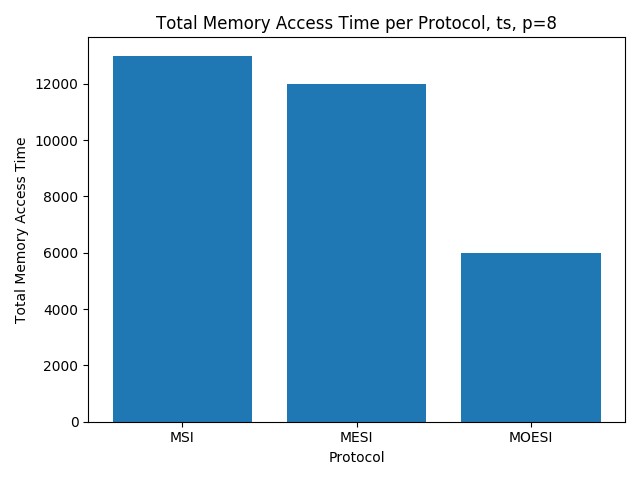
\includegraphics[width=.5\textwidth]{figures/bst_ts_mem_time.png}
\caption{MOESI outperforms other protocols with \inline{ts} on BST program}
\label{fig:bst}
\end{figure}

\section{Conclusion}

Our findings above illustrate that effectiveness of our cache simulator in analysing parallel programs and different cache coherence protocols.  Through the statistics provided by the simulator, we found that aligned arraylocks far outperform the other lock types we implementedin terms of cache performance, at the cost of higher memory utilization.  However, our simulator estimates that test-and-test-and-set locks operate at roughly the same overall latency as the arraylock due to lower cost of acquiring/releasing the lock.  Our findings also demonstrate the benefits of the MOESI cache protocol over the MESI and MSI protocols, due to the great reduction in main memory accesses under certain workloads.

Overall, we feel the project allowed us to explore interesting ideas discussed in class in more depth, and gave us a greater understanding of the importance of writing cache-friendly code, especially on multiprocessor shared address space machines.


\section{References}
\href{http://www.cs.cmu.edu/afs/cs/academic/class/15418-f20/public/lectures/10\_cachecoherence1.pdf}{http://www.cs.cmu.edu/afs/cs/academic/class/15418-f20/public/lectures/10\_cachecoherence1.pdf} \\
\href{http://www.cs.cmu.edu/afs/cs/academic/class/15418-f20/public/lectures/11\_directorycoherence.pdf}{http://www.cs.cmu.edu/afs/cs/academic/class/15418-f20/public/lectures/11\_directorycoherence.pdf} \\
\href{http://www.cs.cmu.edu/afs/cs/academic/class/15418-f20/public/lectures/17\_synchronization.pdf}{http://www.cs.cmu.edu/afs/cs/academic/class/15418-f20/public/lectures/17\_synchronization.pdf} \\
\href{https://en.wikipedia.org/wiki/Directory-based\_coherence}{https://en.wikipedia.org/wiki/Directory-based\_coherence} \\
\href{https://people.eecs.berkeley.edu/~ pattrsn/252F96/Lecture18.pdf}{https://people.eecs.berkeley.edu/$\sim$pattrsn/252F96/Lecture18.pdf} \\

D. Lenoski, J. Laudon, K. Gharachorloo, A. Gupta and J. Hennessy, "The directory-based cache coherence protocol for the DASH multiprocessor," [1990] Proceedings. The 17th Annual International Symposium on Computer Architecture, Seattle, WA, USA, 1990, pp. 148-159, doi: 10.1109/ISCA.1990.134520.

\section{Work Distribution}

\subsection{Task Breakdown}
\begin{table}[H]
    \centering
    \renewcommand{\arraystretch}{1.5}
    \begin{tabular}{| p{.5\linewidth} | c |}
        \hline
        \textbf{Task} & \textbf{Performed By} \\
        \hline \hline
        Making the proposal doc & Sam \\
        \hline
        Writing the entire simulator & Sam \\
        \hline
        Making the checkpoint doc & Sam \\
        \hline
        Writing a script to generate all traces and run simulations on each & Sam \\
        \hline
        Writing the pin tool & Brian \\
        \hline
        Writing lock implementations and parallel BST & Brian \\
        \hline
        Writing a script to generate plots for simulator output & Brian and Sam \\
        \hline
        Writing the final doc & Brian and Sam \\
        \hline
        Making final presentation & Sam \\
        \hline
    \end{tabular}
\end{table}

\subsection{Final Distribution}
\textbf{Sam: } x\% \\
\textbf{Brian: } y\%


\end{document}


